\documentclass[fr]{../../../../../../eplexam}
\usepackage{../../../../../../eplunits}
\usepackage{caption}
\usepackage{subcaption}
\usepackage[american]{circuitikz}

\hypertitle{Circuits électroniques}{5}{ELEC}{1530}{2018}{Janvier}{Mineure}
{Martin Braquet \and Alice Borbath}
{Denis Flandre et Jean-Didier Legat}

\section{Théorie Flandre}

Schéma MOS en grille commune

\begin{enumerate}
    \item Quels sont les types de montage et circuit ?
    \item Expliquez ce qu'est chacun des éléments du circuit et son rôle dans celui-ci.
    \item Dessinez le schéma petit-signal complet. Calculez et définissez ensuite les résistances $R_{in}$, $R_{out}$ et \textbf{les} gains dans la bande passante.
    \item Calculez un pôle basse fréquence et un pôle haute fréquence.
    \item Dessinez le diagramme de Bode de ce circuit et définissez-le.
\end{enumerate}

\section{Théorie Legat}

\begin{enumerate}
    \item Expliquez ce qu'est la D-FF et son fonctionnement en 2-3 lignes. Définissez ensuite ce que sont le \textit{setup time} et le \textit{hold time}.
    \item Dessinez une porte logique XOR de la manière la plus optimale et établissez la table de vérité.
    \item Décrivez et expliquez le fonctionnement du schéma entouré (transistor monté en diode entouré).
    \begin{figure}[h!]
  \begin{center}
    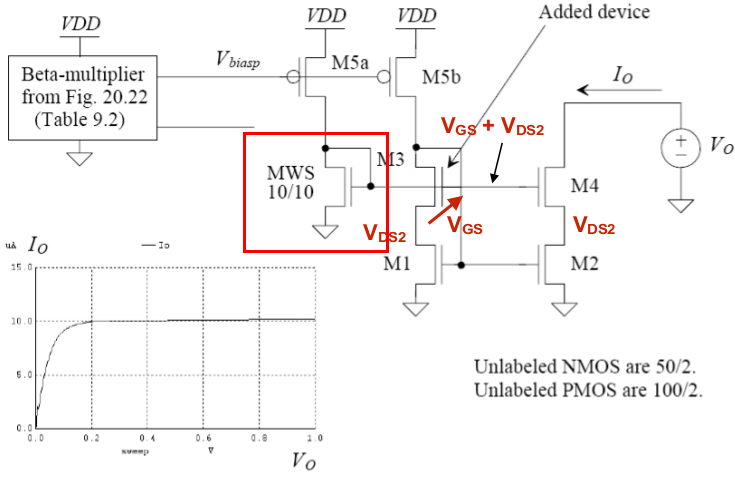
\includegraphics[scale=0.3]{legat1} 
    \caption{Schéma du circuit}
  \end{center}
\end{figure}

    \item Dessinez le schéma d'une paire différentielle avec le miroir de courant et définissez le gain de celle-ci.
\end{enumerate}

\section{Exercice Flandre}

Transistor bipolaire, $v_{in}$ à la base, reliée à $C_1$ et puis diviseur résistif de deux résistances de $100k\Omega$, $v_{out1}$ à l'émetteur, relié à $C_3$ et tension d'émetteur descend vers la masse par $R_E$ et une source de courant I, $v_{out2}$ au collecteur relié à $C_2$ et monte vers $V_{CC}$ par la résistance $R_C$. $R_C=2.15k\Omega$, $R_E=3.4k\Omega$, $C_1=100nF$, $C_2=200nF$, $C_3=400nF$, $C_\pi=$, $V_{CC}=10V$.

\begin{enumerate}
    \item Calculez tous les courants et tensions en DC.
    \item Calculez les gains ($v_{out1}/v_{in}$) et ($v_{out2}/v_{in}$) dans la bande passante.
    \item Calculez les résistances de sortie $R_{out1}$ et $R_{out2}$, ainsi que la résistance d'entrée $R_{in}$.
    \item Calculez tous les pôles basse fréquence.
    \item Calculez le pôle haute fréquence dû à la capacité $C_\pi$.
    \item Dessinez le diagramme de Bode.
    \item Recalculez le gain ($v_{out2}/v_{in}$) si $v_{out1}$ est à la masse.
\end{enumerate}

\section{Exercice Legat}

\begin{enumerate}
    \item Définissez la logique utilisée dans ce circuit. Expliquez brièvement son fonctionnement.
    \item Quelle est la fonction implémentée ? Vérifiez par une table de vérité.
    \item Dimensionnez les transistors sur base du transistor unitaire, $(W/L)_n=10$ et $(W/L)_p=20$, et expliquez votre raisonnement.
    \item Calculez le délai à 50\% entre $(A, B, C, CLK)=(1, 0, 1, 1)$ à $(A, B, C, CLK)=(1, 0, 1, 0)$.
\end{enumerate}

\begin{figure}[h!]
	\centering
	\begin{subfigure}[t]{0.4\textwidth}
		\centering
		\begin{circuitikz}[ scale=1, american voltages]\draw[thick]
			(0,8) node[pmos](pmos1){}
			(3,4) node[pmos](pmos2){}
			(1,6) node[pmos](nmos3){}
			(-1,6) node[pmos](nmos2){}
			(0,2) node[nmos](nmos1){}
			(0,4) node[pmos](nmos4){}
			(3,2) node[nmos](nmos5){}
			(pmos1.S) --++(0,0) node[vdd]{VDD}
			(pmos2.S) --++(0,0) node[vdd]{VDD}
			(nmos1.S) -- (0,1)
			(0,1) node[sground] {}
			(3,1) node[sground] {}
			(nmos1.G) node[anchor=east] {$CLK$}
			(nmos2.G) node[anchor=east] {$A$}
			(nmos3.G) node[anchor=east] {$B$}
			(nmos4.G) node[anchor=east] {$C$}
			(pmos1.G) node[anchor=east] {$CLK$}
			(1,3) node[anchor=south] {$X$}
			(4,3) node[anchor=east] {$Y$}
			(3,3) -- (3.5,3)
			(3,1) -- (nmos5.S)
			(0,3) -- (2,3)
			(2,2) -- (2,4)
			%(nmos5.G) -- (2,1)
			%(pmos2.G) -- (2,8)
			(nmos5.D) -- (pmos2.D)
			(0,7) -- (pmos1.D)
			(-1,5) to[short] (1,5)
			(nmos2.S) to[short] (-1,7)
			(nmos4.S) to[short] (0,5)
			(nmos3.S) to[short] (1,7)
			(nmos4.D) to[short] (0,3)
			(-1,7) to[short] (1,7)
			(nmos2.D) to[short] (-1,5)
			(nmos3.D) to[short] (1,5)
			(nmos1.D) to[short] (0,3);
			\end{circuitikz}
		\caption{Circuit}
	\end{subfigure}
	%
	\begin{subfigure}[t]{0.4\textwidth}
		\centering
		\begin{circuitikz}[ scale=1, american voltages]\draw[thick]
			(3,8) node[pmos](pmos2){}
			(3,6) node[nmos](nmos5){}
			(pmos2.S) --++(0,0) node[vdd]{VDD}
			(3,7) -- (3.5,7)
			(2,7) -- (1.5,7)
			(nmos5.D) -- (pmos2.D)
			(2,6) -- (2,8)
			(nmos5.G) -- (2,6)
			(pmos2.G) -- (2,8)
			(3,5) -- (nmos5.S)
			(nmos5) node[anchor=west]{10/1}
			(pmos2) node[anchor=west]{20/1}
			(3,5) node[sground] {}
			;
		\end{circuitikz}
		\caption{Inverseur unitaire}
	\end{subfigure}
	\caption{Circuits de la question 2.2}
\end{figure}

\begin{solution}

\begin{enumerate}
    \item Logique DOMINO de type P. On charge Y quand $CLK=1$ et puis on évalue Y quand $CLK=0$. 
    \item $CLK+A\cdot B+C$.
    \item $$(W/L)_{CLK,n}=10/1$$
	  $$(W/L)_{CLK,p}=(W/L)_A=(W/L)_B=(W/L)_C=60/1$$
	  Les transistors de l'inverseur qui suit sont dimensionnés comme l'inverseur unitaire.
    \item 
    Calculons le temps de charge de $X$, puis le temps de décharge de $Y$ : 
    \begin{itemize}
        \item Pour $t_{PLH,1}$, nous avons 3 transistors PMOS en série de taille $60/1$ : $N=3$ et $R_p=\SI{68/60}{\kilo\Omega}$. Dès lors,
        $$t_{PLH,1} = 0.7 \cdot 3 \cdot C_{load} \cdot R_p + 0.35 \cdot 3^2 \cdot R_p \cdot C_{oxp}$$
        où $$C_{load}=\frac{3}{2}(C_{oxn,inv}+C_{oxp,inv})+C_{oxn,CLK}=\frac{3}{2} \cdot (20+10) \cdot 62.5\cdot 10^{-18}+10 \cdot 62.5\cdot 10^{-18}=\SI{3.4375}{\femto\farad}$$ et $$C_{oxp}=60\cdot62.5\cdot 10^{-18}=\SI{3.75}{\femto\farad}$$
        On a donc $t_{PLH,1}=\SI{21.56875}{\pico\second}$.
        \item Pour $t_{PHL,2}$, nous considérons le transistor NMOS car il décharge $Y$. Dès lors, $$t_{PHL,2} = 0.7 \cdot C_{load} \cdot R_n$$ où $$C_{load}=C_L+C_{oxn,inv}+C_{oxp,inv}=20\cdot 10^{-15}+(10+20)\cdot 62.5 \cdot 10^{-18}=\SI{21.875}{\femto\farad}$$
        On a donc $t_{PHL,2}=\SI{52.0625}{\pico\second}$.
    \end{itemize}
    Finalement, $t_{PHL} =t_{PLH,1}+t_{PHL,2} = \SI{73.63125}{\pico\second}$.
\end{enumerate}

\end{solution}

\end{document}
